\documentclass{article}

\usepackage{amsfonts}
\usepackage{amsmath}
\usepackage{interval}
\usepackage[T1]{fontenc}
\usepackage{pdftexcmds}
\usepackage{minted}
\usepackage{pgfplots}
\pgfplotsset{compat=1.8}

\begin{document}

\title{A Model of Double-Entry Bookkeeping Systems}
\author{}
\date{}
\maketitle

\section{Double-Entry Bookkeeping Space}

A double-entry bookkeeping information system can be viewed as a three dimensional space,
where each dimension represents:

\begin{itemize}
	\item $a \in A$, where $A$ is a subset of a predefined set of accounts.
	\item $d \in D$, where $D$ is a subset of all possible dates
		in the Gregorian calendar.
	\item $m \in M$, where $M$ is a subset of all possible discrete points in time, given a precision.
\end{itemize}

Figure~\ref{fig:deb-space-sample} shows a \emph{double-entry bookkeeping space} sample, 
where each cube represents a integer value different from zero.
Consider the cubes $(4,1,1)$ and $(6,1,1)$. They share the same moment 
and date---the only difference are the accounts. 
We can interpret this pair of cubes as a transaction recorded in the system,
with one cube representing the debit and another representing the credit.

\begin{figure}[h]
\centering
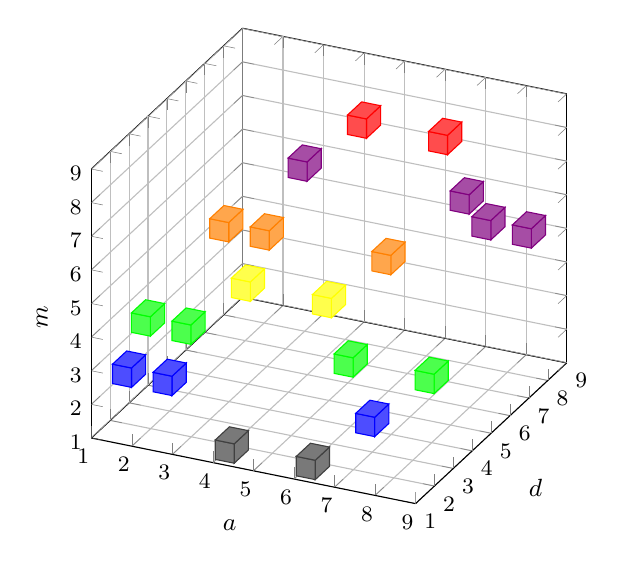
\begin{tikzpicture}
\begin{axis}[
	% view={120}{40},
	small,
	height=3in,
	width=3in,
	grid=major,
	xlabel=$a$,
	ylabel=$d$,
	zlabel=$m$,
	xmin=1,xmax=9,
    ymin=1,ymax=9,
    zmin=1,zmax=9,
    xtick={1,2,...,10},
    ytick={1,2,...,10},
    ztick={1,2,...,10},
	colormap={summap}{
        color=(darkgray); color=(blue);
        color=(green); color=(yellow)
        color=(orange) color=(violet)
        color=(red)
    },
    scatter/use mapped color={
        draw=mapped color,fill=mapped color!70},
]
\addplot3[only marks,scatter,mark=cube*,mark size=7] coordinates {
            (4,2,1) (6,2,1) 
            (7,3,2) (1,3,2) (2,3,2)
            (1,4,3) (2,4,3) (6,4,3) (8,4,3)
            (3,5,4) (5,5,4) 
            (3,6,5) (6,6,5) (2,6,5)
            (8,7,6) (9,7,6) (3,8,6) (7,8,6)
            (4,9,7) (6,9,7)
        };
\end{axis}
\end{tikzpicture}
\label{fig:deb-space-sample}
\caption{A \emph{double-entry bookkeeping space} sample.}
\end{figure}

As, by definition, a double-entry transaction must have debits' sum
equals to credits' sum, we can deduce that the values for both
cubes are the same, in this example.

More specifically, we can have a \emph{double-entry bookkeeping space} 
represented by a three dimensional array $S$:
\begin{equation}
	\label{eq:space}
	S = \left(s_{ijk}\right), 
	\; 1 \leq i \leq |A|, \; 1 \leq j \leq |D|, \; 1 \leq k \leq |M|, 
	\; s_{ijk} \in \mathbb{Z}
\end{equation}

Satisfying the following property:

\begin{equation}
	\label{eq:property}
	\forall j \; \forall k, \sum_{i=1}^{|A|}{s_{ijk}} = 0
\end{equation}

The equations~\eqref{eq:space}~and~\eqref{eq:property}
assume that debits are represented by positive integers
and credits by negative integers.

\section{Operations}

In the following description of the operations, the notation $\langle x, y \rangle$ means
a range specification, and $R^{\langle n \rangle}$ means a set of $n$
range specifications.

A \emph{double-entry bookkeeping space} supports the following operations:

\begin{description}
	\item[\textsc{Append}$(S,S')$] append the space
	$S'=\left(s'_{ijk}\right)$ to the space $S$,
		such that, given the set $M$ associated with the space $S$ and
		the set $M'$ associated with the space $S':
		M \cap M' = \emptyset$, and
		\[
			s_{ij(|M|+k)} = s'_{ijk}, \; 1 \leq k \leq |M'|.
		\]
		The new set $M \cup M'$ will be the new set associated with $S$
		instead of $M$.

	\item[\textsc{Projection}$(S, D^{\langle n \rangle}, M^{\langle m \rangle})$] 
		returns a potentially smaller space $S'=\left(s'_{pqr}\right)$,
		where $D^{\langle n \rangle} = \{\langle x_i, y_i \rangle\}$, and
		$M^{\langle m \rangle} = \{\langle u_i, w_i \rangle\}$,
		such that:
		\begin{align*}
			s'_{pqr} &= \sum_{j=x_q}^{y_q}{\sum_{k=u_r}^{w_r}{s_{pjk}}} \\ 
			1 \leq & \; p \leq |A| \\
			1 \leq & \; q \leq n \\
			1 \leq & \; r \leq m.
		\end{align*}

	\item[\textsc{Slice}$(S, A', D^{\langle n \rangle}, M^{\langle m \rangle})$] 
		returns a potentially smaller space $S'=\left(s'_{pqr}\right)$, 
		where $D^{\langle n \rangle} = \{\langle x_i, y_i \rangle\}$, and
		$M^{\langle m \rangle} = \{\langle u_i, w_i \rangle\}$,
		such that:
		\begin{align*}
			s'_{pqr} & = s_{pjk} \\
			1 \leq & \; p \leq |A| \\
			1 \leq & \; q \leq \sum_{i=1}^{n}{y_i-x_i+1} \\
			1 \leq & \; r \leq \sum_{i=1}^{m}{w_i-u_i+1} \\
			x_i \leq & \; j \leq y_i, \forall i \in \{1,\cdots,n\} \\
			u_i \leq & \; k \leq w_i, \forall i \in \{1,\cdots,m\} \\
			\forall A_{p} \in A' & \quad s'_{pqr} \neq 0.
		\end{align*}

\end{description}

\section{Alloy Model} % (fold)
\label{sec:alloy_model}

\inputminted{alloy}{model.als}%

% section alloy_model (end)

\end{document}